\chapter{ADR Dataset and Extraction}

    \section{Data collection Process}
        The dataset used for the study was obtained from a previous MSR study\cite{Github_study_ADRs}. The researchers preformed an exhaustive search on GitHub in 2020 which included going through all registered platform users to find public repositories that contained files that matched various template formats of ADRs. After this process was completed, the repositories were also verified manually according to rigorous inclusion and exclusion criteria. The resulting dataset contained metadata for 6362 ADRs from 921 software repositories. However, since the researchers focused mainly on measuring trends and use of ADRs, only the metadata were stored and made publicly available in a separate GitHub repository\footnote{https://github.com/software-competence-center-hagenberg/ADR-Study-Dataset}. The dataset files, one for each repository, were stored in a JSON format and contained information about the repository such as its hyperlink, the number and path of ADR directories, and detailed metadata for each ADR as seen in figure 5.1\ref{fig:JSON_data}. This metadata included the directory path, file path, type of ADR template used, status, timestamps of the first and last commits, the number of commits, and details about the authors. Because of the need to focus on the contents of each ADR, each repository needed to be cloned (downloaded) and the ADRs to be extracted from the specified folder as mentioned in the metadata. This also accounted for newly created ADRs after the date the data was scrapped since the projects may have continued their use even after the study was published. It is important to note that some GitHub repositories (~20) were deleted, which prevented their inclusion in the dataset. The whole was done in an automated way via a Python script. The final contents of the respective folders were saved and examined.

        \begin{figure}[]
            \centering
            \includegraphics[scale=0.4]{figures/JSON_data_example.png}
            \caption{Example of a JSON metadata file derived from the base dataset.}
            \label{fig:JSON_data}
        \end{figure}
        
    \section{Data Cleaning and Enrichment}
        After the contents of the ADR folders were obtained, at first, the files needed to undergo a cleaning process. I decided to include only markdown files since they comprised the vast majority of the actual files downloaded at a percentage of more than 98 percent and was the dominant file type for the ADRs as proposed in the Markdown Architectural Decision Records \cite{MarkdownADRs} article. This also eliminated exogenous files such as any source code that was stored in the folders in question. Next, irrelevant files and files related to ADRs that did not provide any actual information of use needed to be deleted such as licences, ADR templates, contributing guides and "README" files. ADR drafts and examples were also excluded since they did not relate to any specific topic. This procedure was also executed automatically via Python scripts and it resulted in 5368 ADRs markdown files.

        The final cleaning process was performed on the ADR text itself to reduce language-dependent factors in order for the topic modelling analysis to produce more coherent results. Text is generally written in natural language for human understanding, but in text mining, this data is not always straightforward for computers to process as it frequently contains words and other elements that provide no information gain to algorithms and models. Therefore, it is common practice in topic modelling, for text to undergo preprocessing where specific tokens from documents are usually removed. \cite{topic-modelling-text-cleaning, text-mining-lda}. In this case, all non-alphabetic characters were removed and all text was converted to lower case. In addition, stop words, stemmed from the ntlk natural language toolkit Python library were also removed as they were deemed insignificant. These included pronouns in many forms from a commonly used list of 127 entries\footnote{https://gist.github.com/sebleier/554280}. Furthermore, all words with less than 3 characters were also filtered out and all remaining words were lemmatized or reduced to their base or root form, by removing inflections and derivational suffixes, ensuring that related forms of a word are treated as a single item. Finally, a list of unwanted terms was manually assembled after careful examination of a subset of documents. This list included words from common ADR template titles such as "context", "decision", "status", "consequences", "motivation", "options", "option", "alternatives" and others, that were present in almost all documents and did not provide any context on their topics, but instead were used to honor the ADR format. Other common but unwanted words included the name of the proposer of a popular ADR template "Michael Nygard" \footnote{https://cognitect.com/blog/2011/11/15/documenting-architecture-decisions} and were also filtered out. Code-specific stopwords such as "class," "interface" and "abstract" were not removed as to provide information about the implementation of the decision. The final form of each document was reduced to a series of words that captured the semantic properties and general meaning of the architectural decision. An example cleaned ADR can be seen in figure \ref{fig:Cleaned_ADR} and an overview of the cleaning process in figure \ref{fig:Data_cleaning_steps}
        
        \begin{figure}[]
            \centering
            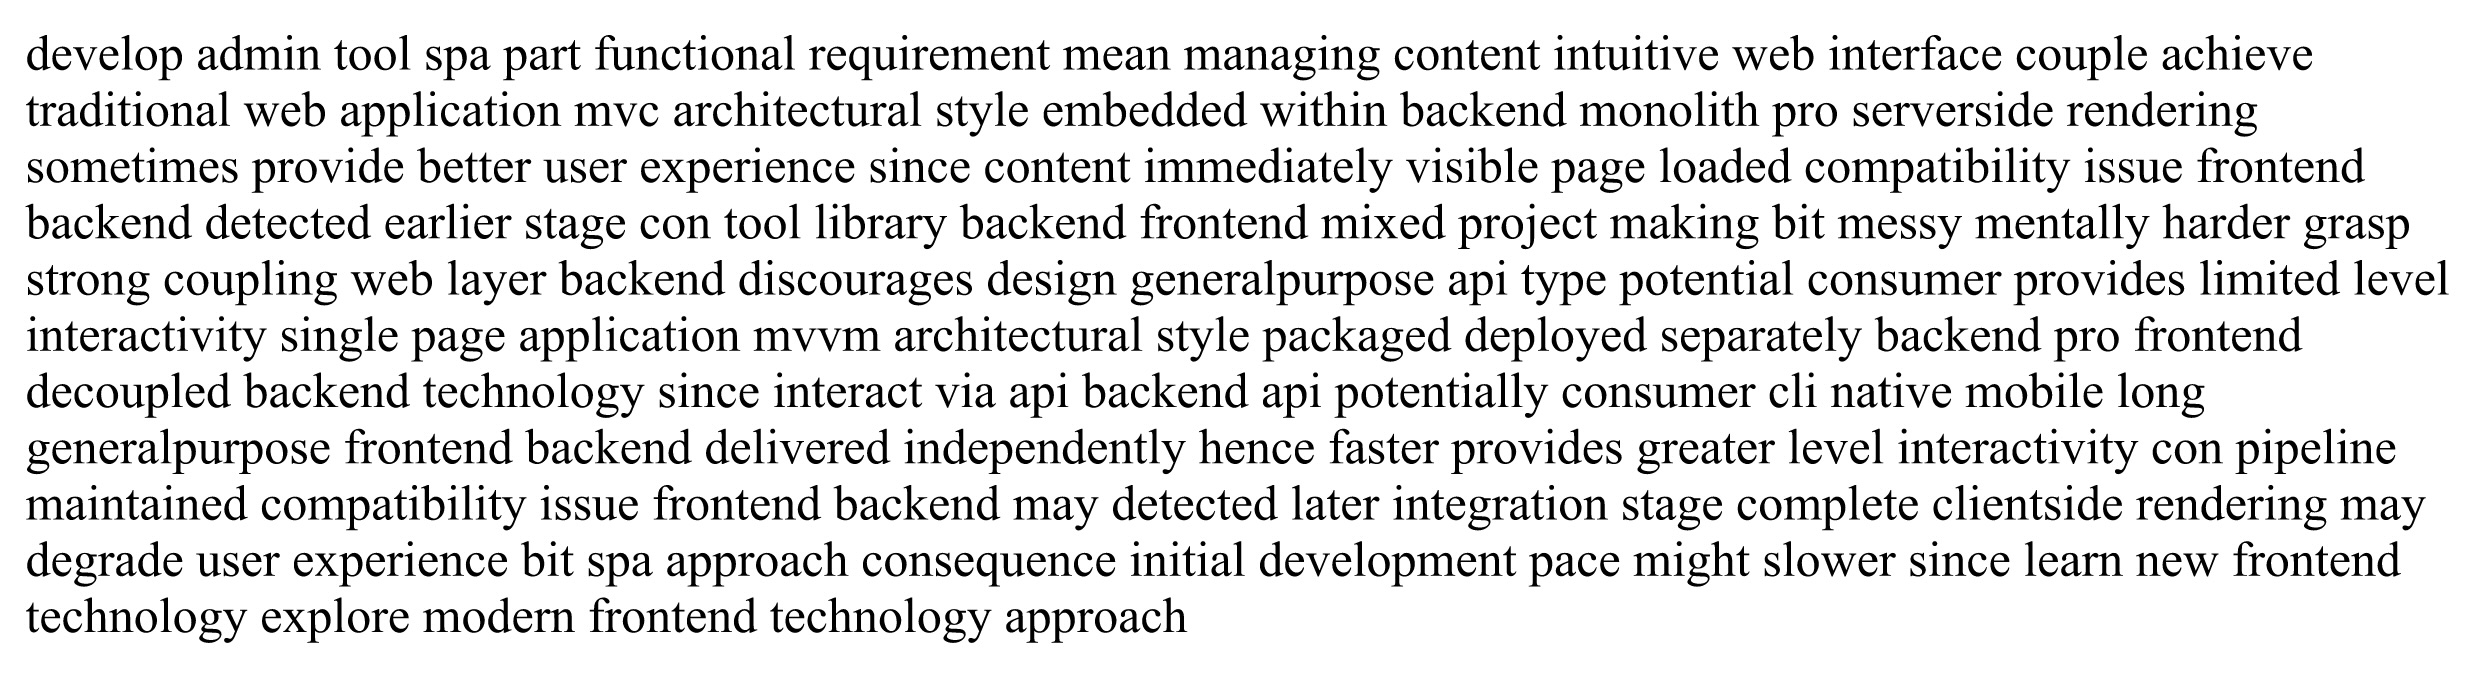
\includegraphics[scale=0.6]{figures/adr_cleaned_example.jpeg}
            \caption{Example of an ADR about creating a web interface after undergoing preprocessing.}
            \label{fig:Cleaned_ADR}
        \end{figure}

        \begin{figure}[ht]
            \centering
            % \fontsize{7}{8}\selectfont
            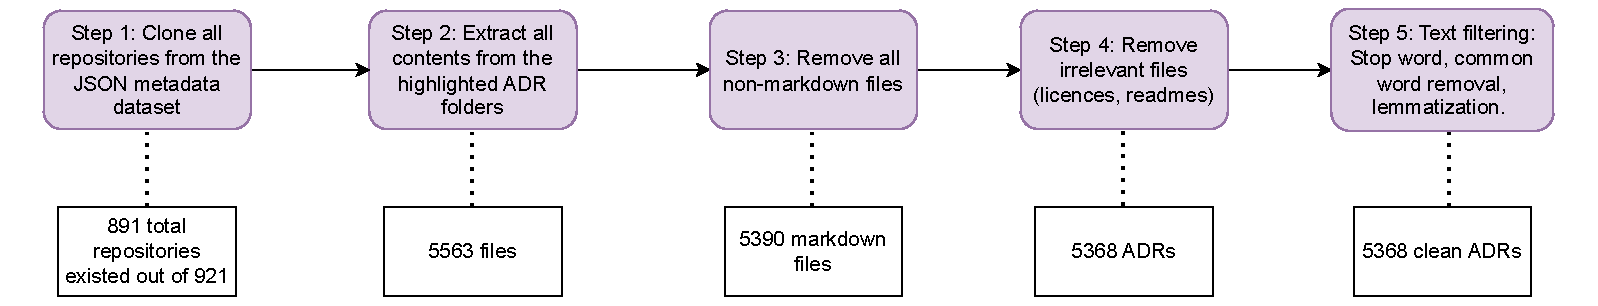
\includegraphics[width=\textwidth]{figures/data_cleaning_steps_final2.pdf}
            \caption{Data cleaning process.}
            \label{fig:Data_cleaning_steps}
        \end{figure}
        
    \section{Dataset Validity and Quality}
    While this dataset provides a valuable snapshot of ADR usage in open-source projects, several validity and quality concerns need to be addressed. Firstly, despite it being derived from a broad search on all GitHub repositories, the final sample size remains small. There exist a plethora of reasons for why this may be observed. ADRs are not yet widely adopted, which is understandable since they were introduced recently, with the earliest ADR commit in the dataset dating back to May 2013. Furthermore, it is possible that many ADRs remain private, either in private code repositories or internal company documentation, not found on any code hosting platforms. The later can be confirmed by the statements of companies like Spotify and Amazon, as mentioned in chapter 3, that choose to keep code proprietary and records private.
    In addition, in regards to ADR content and selection, potential over-filtering might have removed relevant information, and the manual assembly of unwanted terms introduces an element of subjectivity. In contrast, it is possible that records and phrases that provide no additional meaning were not filtered and a more thorough approach of examining the records before cleaning them is needed. To promote dataset quality, future research could include expanding the dataset size with private records, or public ADRs that are not stored on GitHub and refining the cleaning process to mitigate these limitations.